% This file was created by matlab2tikz.
%
%The latest updates can be retrieved from
%  http://www.mathworks.com/matlabcentral/fileexchange/22022-matlab2tikz-matlab2tikz
%where you can also make suggestions and rate matlab2tikz.
%
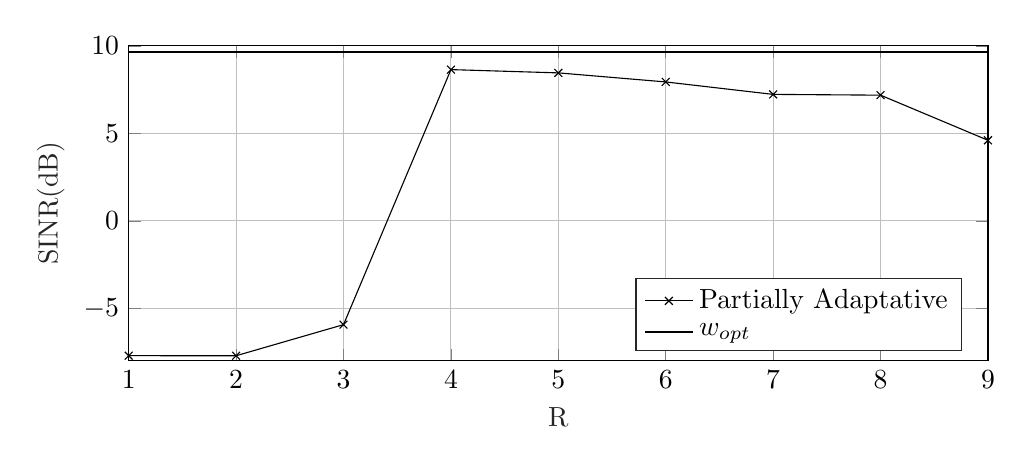
\begin{tikzpicture}

\begin{axis}[%
width=.9\linewidth,
height=4cm,
at={(0in,0in)},
scale only axis,
xmin=1,
xmax=9,
xlabel style={font=\color{white!15!black}},
xlabel={R},
ymin=-8,
ymax=10,
ylabel style={font=\color{white!15!black}},
ylabel={SINR(dB)},
axis background/.style={fill=white},
xmajorgrids,
ymajorgrids,
legend style={at={(0.97,0.03)}, anchor=south east, legend cell align=left, align=left, draw=white!15!black}
]
\addplot [color=black, mark=x, mark options={solid, black}]
  table[row sep=crcr]{%
1	-7.70875975669615\\
2	-7.71216513418879\\
3	-5.93505069079119\\
4	8.64010011888351\\
5	8.4529353234859\\
6	7.93529221140863\\
7	7.2240981299773\\
8	7.17967881225924\\
9	4.60160891751099\\
};
\addlegendentry{Partially Adaptative}

\addplot [color=black, line width=0.7pt]
  table[row sep=crcr]{%
1	9.66056569974277\\
2	9.66056569974277\\
3	9.66056569974277\\
4	9.66056569974277\\
5	9.66056569974277\\
6	9.66056569974277\\
7	9.66056569974277\\
8	9.66056569974277\\
9	9.66056569974277\\
};
\addlegendentry{$\text{w}_{\text{opt}}$}

\end{axis}
\end{tikzpicture}%